% Generated on 2025-04-15 16:10:16 by gEcon ver. 1.2.1 (2023-01-18)
% http://gecon.r-forge.r-project.org/

% Model name: NK_RS

\section{Steady-state values}


\begin{tabular}{c|c|}
  & Steady-state value\\
\hline
$\epsilon^{\mathrm{G}}$ & 1 \\
$g^{\mathrm{1}}$ & 7.3514 \\
$g^{\mathrm{2}}$ & 4.9009 \\
${i\!n\!f\!l\!a\!t\!i\!o\!n}^{\mathrm{gap}}$ & 1 \\
$\lambda$ & 1.5467 \\
${m\!c}$ & 0.6667 \\
$\nu^{\mathrm{p}}$ & 1 \\
${p\!e\!r\!c\!i\!e\!v\!e\!d}^{\pi^{\mathrm{obj}}}$ & 1 \\
$\pi$ & 1 \\
$\pi^{\star}$ & 1 \\
$\pi^{\mathrm{obj}}$ & 1 \\
${p\!H}$ & 0.95 \\
${p\!L}$ & 0.05 \\
$q$ & 1.5467 \\
$r$ & 0.0351 \\
$B$ & 0 \\
$C$ & 0.3255 \\
${D\!i\!v}$ & 0.1601 \\
$G$ & 0.0865 \\
$I$ & 0.0684 \\
$K^{\mathrm{s}}$ & 2.7374 \\
$L^{\mathrm{s}}$ & 0.2279 \\
$Q$ & 1 \\
$R$ & 1.0101 \\
$T$ & 0.0865 \\
$U$ & -167.8256 \\
$W$ & 0.9837 \\
$Y$ & 0.4804 \\
$Y^{\mathrm{j}}$ & 0.4804 \\
$Y^{\mathrm{s}}$ & 0.4804 \\
$Z$ & 1 \\
\hline
\end{tabular}


\section{The solution of the 1st order perturbation}

\subsection*{Matrix $P$}

$$\bordermatrix{
~ & \epsilon^{\mathrm{G}}_{t-1} & \nu^{\mathrm{p}}_{t-1} & {p\!e\!r\!c\!i\!e\!v\!e\!d}^{\pi^{\mathrm{obj}}}_{t-1} & \pi_{t-1} & \pi^{\mathrm{obj}}_{t-1} & B_{t-1} & K^{\mathrm{s}}_{t-1} & R_{t-1} & Z_{t-1} \cr
\epsilon^{\mathrm{G}}_{t} & 0.949 & 0 & 0 & 0 & 0 & 0 & 0 & 0 & 0 \cr
\nu^{\mathrm{p}}_{t} & 0 & 0.908 & 0 & 0 & 0 & 0 & 0 & 0 & 0 \cr
{p\!e\!r\!c\!i\!e\!v\!e\!d}^{\pi^{\mathrm{obj}}}_{t} & 0 & 0.0002 & 0.0498 & 0.0014 & 0.0015 & 0 & -0.0002 & -0.0047 & -0.0003 \cr
\pi_{t} & -0.0001 & 0.0549 & 0.0015 & 0.3348 & 0.3434 & 0 & -0.0399 & -1.1153 & -0.0645 \cr
\pi^{\mathrm{obj}}_{t} & 0 & 0 & 0.0038 & 0.0001 & 0.9241 & 0 & 0 & -0.0004 & 0 \cr
B_{t} & 0 & 0 & 0 & 0 & 0 & 0 & 0 & 0 & 0 \cr
K^{\mathrm{s}}_{t} & 0.0052 & 0.553 & 0.0151 & -1.2485 & 3.509 & 0 & 0.4383 & -15.1027 & -0.4035 \cr
R_{t} & 0.0006 & 0.0147 & 0.0003 & 0.0313 & 0.0718 & 0 & -0.0135 & 0.5465 & -0.011 \cr
Z_{t} & 0 & 0 & 0 & 0 & 0 & 0 & 0 & 0 & 0.823 \cr
}$$

\subsection*{Matrix $Q$}

$$\bordermatrix{
~ & \epsilon^{\mathrm{Z}} & \eta^{\mathrm{p}} & \eta^{\mathrm{R}} & \eta^{\pi} & \eta^{\mathrm{G}} \cr
\epsilon^{\mathrm{G}} & 0 & 0 & 0 & 0 & 1 \cr
\nu^{\mathrm{p}} & 0 & 0 & 0 & 0 & 0 \cr
{p\!e\!r\!c\!i\!e\!v\!e\!d}^{\pi^{\mathrm{obj}}} & -0.0003 & 0.0001 & -0.0049 & 0.0016 & 0 \cr
\pi & -0.0783 & 0.0121 & -1.1605 & 0.3716 & -0.0001 \cr
\pi^{\mathrm{obj}} & 0 & 0 & -0.0004 & 1.0001 & 0 \cr
B & 0 & 0 & 0 & 0 & 0 \cr
K^{\mathrm{s}} & -0.4903 & -0.0064 & -15.7156 & 3.7977 & 0.0055 \cr
R & -0.0133 & -0.0002 & 0.5686 & 0.0777 & 0.0007 \cr
Z & 1 & 0 & 0 & 0 & 0 \cr
}$$

\subsection*{Matrix $R$}

$$\bordermatrix{
~ & \epsilon^{\mathrm{G}}_{t-1} & \nu^{\mathrm{p}}_{t-1} & {p\!e\!r\!c\!i\!e\!v\!e\!d}^{\pi^{\mathrm{obj}}}_{t-1} & \pi_{t-1} & \pi^{\mathrm{obj}}_{t-1} & B_{t-1} & K^{\mathrm{s}}_{t-1} & R_{t-1} & Z_{t-1} \cr
g^{\mathrm{1}}_{t} & 0.1474 & 0.9169 & 0.0235 & -1.976 & 5.4626 & 0 & -0.8828 & -15.6845 & -0.8633 \cr
g^{\mathrm{2}}_{t} & 0.1474 & 0.9169 & 0.0235 & -1.976 & 5.4626 & 0 & -0.8828 & -15.6845 & -0.8633 \cr
{i\!n\!f\!l\!a\!t\!i\!o\!n}^{\mathrm{gap}}_{t} & -0.0001 & 0.0547 & -0.0483 & 0.3334 & 0.3419 & 0 & -0.0398 & -1.1105 & -0.0642 \cr
\lambda_{t} & 0.118 & 0.1357 & -0.0094 & 0.804 & -2.192 & 0 & -0.2745 & 9.2064 & -0.0383 \cr
{m\!c}_{t} & 0.086 & 4.973 & 0.123 & -10.2094 & 28.5968 & 0 & -4.1819 & -122.7528 & -4.7432 \cr
\pi^{\star}_{t} & -0.0012 & 0.5422 & 0.0146 & -1.3243 & 3.3889 & 0 & -0.3942 & -11.0072 & -0.6364 \cr
{p\!H}_{t} & 0 & -0.0027 & 0.0024 & -0.0167 & -0.0171 & 0 & 0.002 & 0.0555 & 0.0032 \cr
{p\!L}_{t} & -0.0001 & 0.052 & -0.0459 & 0.3167 & 0.3248 & 0 & -0.0378 & -1.055 & -0.061 \cr
q_{t} & 0.118 & 0.1357 & -0.0094 & 0.804 & -2.192 & 0 & -0.2745 & 9.2064 & -0.0383 \cr
r_{t} & 0.2501 & 9.6861 & 0.2305 & -19.112 & 53.5762 & 0 & -8.6812 & -230.1222 & -7.5864 \cr
C_{t} & -0.0535 & 0.9657 & 0.0317 & -2.6399 & 7.358 & 0 & -0.6515 & -31.4613 & -0.803 \cr
{D\!i\!v}_{t} & -0.008 & -7.957 & -0.1386 & 11.5161 & -32.2143 & 0 & 4.8645 & 138.1362 & 6.6432 \cr
G_{t} & 0.949 & 0 & 0 & 0 & 0 & 0 & 0 & 0 & 0 \cr
I_{t} & 0.2069 & 22.1186 & 0.6037 & -49.9414 & 140.3617 & 0 & -21.4666 & -604.1071 & -16.1403 \cr
L^{\mathrm{s}}_{t} & 0.2344 & 6.7329 & 0.1535 & -12.718 & 35.6848 & 0 & -5.4276 & -153.3848 & -5.2374 \cr
Q_{t} & 0 & 0 & 0 & 0 & 0 & 0 & 0 & 0 & 0 \cr
T_{t} & 0.949 & 0 & 0 & 0 & 0 & 11.5637 & 0 & 0 & 0 \cr
U_{t} & -0.0107 & -0.0272 & 0.0003 & -0.0234 & 0.0592 & 0 & 0.0226 & -0.1954 & 0.0162 \cr
W_{t} & 0.0157 & 2.9532 & 0.077 & -6.394 & 17.8914 & 0 & -2.2536 & -76.7373 & -2.349 \cr
Y_{t} & 0.1641 & 3.805 & 0.1074 & -8.9026 & 24.9794 & 0 & -3.4993 & -107.3694 & -2.8432 \cr
Y^{\mathrm{j}}_{t} & 0.1641 & 4.713 & 0.1074 & -8.9026 & 24.9794 & 0 & -3.4993 & -107.3694 & -2.8432 \cr
Y^{\mathrm{s}}_{t} & 0.1641 & 4.713 & 0.1074 & -8.9026 & 24.9794 & 0 & -3.4993 & -107.3694 & -2.8432 \cr
}$$

\subsection*{Matrix $S$}

$$\bordermatrix{
~ & \epsilon^{\mathrm{Z}} & \eta^{\mathrm{p}} & \eta^{\mathrm{R}} & \eta^{\pi} & \eta^{\mathrm{G}} \cr
g^{\mathrm{1}} & -1.049 & 0.1095 & -16.321 & 5.9119 & 0.1553 \cr
g^{\mathrm{2}} & -1.049 & -0.0266 & -16.321 & 5.9119 & 0.1553 \cr
{i\!n\!f\!l\!a\!t\!i\!o\!n}^{\mathrm{gap}} & -0.078 & 0.012 & -1.1556 & 0.37 & -0.0001 \cr
\lambda & -0.0465 & 0.0051 & 9.5801 & -2.3722 & 0.1243 \cr
{m\!c} & -5.7633 & -0.0535 & -127.7344 & 30.949 & 0.0906 \cr
\pi^{\star} & -0.7732 & 0.1192 & -11.4539 & 3.6676 & -0.0012 \cr
{p\!H} & 0.0039 & -0.0006 & 0.0578 & -0.0185 & 0 \cr
{p\!L} & -0.0741 & 0.0114 & -1.0978 & 0.3515 & -0.0001 \cr
q & -0.0465 & 0.0051 & 9.5801 & -2.3722 & 0.1243 \cr
r & -9.218 & -0.0995 & -239.4611 & 57.9829 & 0.2635 \cr
C & -0.9757 & -0.0144 & -32.7381 & 7.9632 & -0.0564 \cr
{D\!i\!v} & 8.072 & 0.061 & 143.7421 & -34.864 & -0.0084 \cr
G & 0 & 0 & 0 & 0 & 1 \cr
I & -19.6116 & -0.2544 & -628.6234 & 151.9066 & 0.218 \cr
L^{\mathrm{s}} & -6.3638 & -0.0657 & -159.6096 & 38.6199 & 0.247 \cr
Q & 0 & 0 & 0 & 0 & 0 \cr
T & 0 & 0 & 0 & 0 & 1 \cr
U & 0.0197 & -0.0003 & -0.2033 & 0.0641 & -0.0113 \cr
W & -2.8542 & -0.0338 & -79.8515 & 19.363 & 0.0165 \cr
Y & -3.4547 & -0.046 & -111.7267 & 27.034 & 0.1729 \cr
Y^{\mathrm{j}} & -3.4547 & -0.046 & -111.7267 & 27.034 & 0.1729 \cr
Y^{\mathrm{s}} & -3.4547 & -0.046 & -111.7267 & 27.034 & 0.1729 \cr
}$$


\section{Model statistics}

\subsection{Basic statistics}

\begin{tabular}{c|c|c|c|c|}
  & Steady-state value & Std. dev. & Variance & Loglin\\
\hline
$\epsilon^{\mathrm{G}}$ & 1 & 1.3033 & 1.6986 & Y    \\
$g^{\mathrm{1}}$ & 7.3514 & 20.4293 & 417.3582 & Y    \\
$g^{\mathrm{2}}$ & 4.9009 & 20.4291 & 417.3479 & Y    \\
${i\!n\!f\!l\!a\!t\!i\!o\!n}^{\mathrm{gap}}$ & 1 & 1.2239 & 1.4979 & Y    \\
$\lambda$ & 1.5467 & 12.2835 & 150.8847 & Y    \\
${m\!c}$ & 0.6667 & 127.9284 & 16365.6722 & Y    \\
$\nu^{\mathrm{p}}$ & 1 & 0 & 0 & Y    \\
${p\!e\!r\!c\!i\!e\!v\!e\!d}^{\pi^{\mathrm{obj}}}$ & 1 & 0.0053 & 0 & Y    \\
$\pi$ & 1 & 1.2291 & 1.5108 & Y    \\
$\pi^{\star}$ & 1 & 11.8882 & 141.3285 & Y    \\
$\pi^{\mathrm{obj}}$ & 1 & 1.2961 & 1.6798 & Y    \\
${p\!H}$ & 0.95 & 0.0612 & 0.0037 & Y    \\
${p\!L}$ & 0.05 & 1.1627 & 1.3518 & Y    \\
$q$ & 1.5467 & 12.2835 & 150.8847 & Y    \\
$r$ & 0.0351 & 246.1829 & 60606.0446 & Y    \\
$B$ & 0 & 0 & 0 & N    \\
$C$ & 0.3255 & 30.8502 & 951.733 & Y    \\
${D\!i\!v}$ & 0.1601 & 145.1801 & 21077.2735 & Y    \\
$G$ & 0.0865 & 1.3033 & 1.6986 & Y    \\
$I$ & 0.0684 & 635.6958 & 404109.1599 & Y    \\
$K^{\mathrm{s}}$ & 2.7374 & 20.0074 & 400.2969 & Y    \\
$L^{\mathrm{s}}$ & 0.2279 & 161.275 & 26009.6363 & Y    \\
$Q$ & 1 & 0 & 0 & Y    \\
$R$ & 1.0101 & 0.6891 & 0.4748 & Y    \\
$T$ & 0.0865 & 1.3033 & 1.6986 & Y    \\
$U$ & -167.8256 & 0.5475 & 0.2997 & Y    \\
$W$ & 0.9837 & 77.7172 & 6039.9577 & Y    \\
$Y$ & 0.4804 & 110.7744 & 12270.972 & Y    \\
$Y^{\mathrm{j}}$ & 0.4804 & 110.7744 & 12270.972 & Y    \\
$Y^{\mathrm{s}}$ & 0.4804 & 110.7744 & 12270.972 & Y    \\
$Z$ & 1 & 1.227 & 1.5056 & Y    \\
\hline
\end{tabular}


\subsection{Correlation matrix}

\begin{tabular}{c|cccccccccccccccccccccccccccc|}
  & $\epsilon^{\mathrm{G}}$ & $g^{\mathrm{1}}$ & $g^{\mathrm{2}}$ & ${i\!n\!f\!l\!a\!t\!i\!o\!n}^{\mathrm{gap}}$ & $\lambda$ & ${m\!c}$ & ${p\!e\!r\!c\!i\!e\!v\!e\!d}^{\pi^{\mathrm{obj}}}$ & $\pi$ & $\pi^{\star}$ & $\pi^{\mathrm{obj}}$ & ${p\!H}$ & ${p\!L}$ & $q$ & $r$ & $C$ & ${D\!i\!v}$ & $G$ & $I$ & $K^{\mathrm{s}}$ & $L^{\mathrm{s}}$ & $R$ & $T$ & $U$ & $W$ & $Y$ & $Y^{\mathrm{j}}$ & $Y^{\mathrm{s}}$ & $Z$\\
\hline
$\epsilon^{\mathrm{G}}$ & 1 & 0.009 & 0.009 & -0.001 & 0.013 & 0 & -0.001 & -0.001 & -0.001 & 0 & 0.001 & -0.001 & 0.013 & 0.001 & -0.003 & 0.001 & 1 & 0 & 0 & 0.001 & 0.001 & 1 & -0.027 & 0 & 0.001 & 0.001 & 0.001 & 0 \\
$g^{\mathrm{1}}$ &  & 1 & 1 & 0.771 & -0.134 & 0.94 & 0.742 & 0.771 & 0.958 & 0.148 & -0.771 & 0.771 & -0.134 & 0.959 & 0.828 & -0.947 & 0.009 & 0.948 & 0.142 & 0.947 & -0.121 & 0.009 & -0.312 & 0.909 & 0.931 & 0.931 & 0.931 & -0.031 \\
$g^{\mathrm{2}}$ &  &  & 1 & 0.771 & -0.134 & 0.94 & 0.741 & 0.771 & 0.958 & 0.148 & -0.771 & 0.771 & -0.134 & 0.959 & 0.828 & -0.947 & 0.009 & 0.948 & 0.142 & 0.947 & -0.121 & 0.009 & -0.312 & 0.909 & 0.931 & 0.931 & 0.931 & -0.031 \\
${i\!n\!f\!l\!a\!t\!i\!o\!n}^{\mathrm{gap}}$ &  &  &  & 1 & -0.626 & 0.899 & 0.999 & 1 & 0.888 & 0.284 & -1 & 1 & -0.626 & 0.881 & 0.933 & -0.894 & -0.001 & 0.891 & 0.633 & 0.893 & -0.559 & -0.001 & 0.253 & 0.917 & 0.905 & 0.905 & 0.905 & -0.071 \\
$\lambda$ &  &  &  &  & 1 & -0.445 & -0.641 & -0.626 & -0.411 & -0.244 & 0.626 & -0.626 & 1 & -0.387 & -0.659 & 0.426 & 0.013 & -0.422 & -0.999 & -0.424 & 0.917 & 0.013 & -0.896 & -0.521 & -0.469 & -0.469 & -0.469 & -0.005 \\
${m\!c}$ &  &  &  &  &  & 1 & 0.878 & 0.899 & 0.994 & 0.109 & -0.899 & 0.899 & -0.445 & 0.998 & 0.967 & -1 & 0 & 1 & 0.452 & 1 & -0.449 & 0 & 0.001 & 0.996 & 0.999 & 0.999 & 0.999 & -0.028 \\
${p\!e\!r\!c\!i\!e\!v\!e\!d}^{\pi^{\mathrm{obj}}}$ &  &  &  &  &  &  & 1 & 0.999 & 0.865 & 0.29 & -0.999 & 0.999 & -0.641 & 0.857 & 0.92 & -0.872 & -0.001 & 0.869 & 0.648 & 0.871 & -0.571 & -0.001 & 0.28 & 0.898 & 0.884 & 0.884 & 0.884 & -0.073 \\
$\pi$ &  &  &  &  &  &  &  & 1 & 0.888 & 0.284 & -1 & 1 & -0.626 & 0.881 & 0.933 & -0.894 & -0.001 & 0.891 & 0.633 & 0.893 & -0.559 & -0.001 & 0.253 & 0.917 & 0.905 & 0.905 & 0.905 & -0.071 \\
$\pi^{\star}$ &  &  &  &  &  &  &  &  & 1 & 0.189 & -0.888 & 0.888 & -0.411 & 0.994 & 0.952 & -0.995 & -0.001 & 0.994 & 0.418 & 0.995 & -0.381 & -0.001 & -0.032 & 0.987 & 0.993 & 0.993 & 0.993 & -0.051 \\
$\pi^{\mathrm{obj}}$ &  &  &  &  &  &  &  &  &  & 1 & -0.284 & 0.284 & -0.244 & 0.095 & 0.161 & -0.105 & 0 & 0.103 & 0.238 & 0.104 & 0.16 & 0 & 0.244 & 0.128 & 0.115 & 0.115 & 0.115 & 0 \\
${p\!H}$ &  &  &  &  &  &  &  &  &  &  & 1 & -1 & 0.626 & -0.881 & -0.933 & 0.894 & 0.001 & -0.891 & -0.633 & -0.893 & 0.559 & 0.001 & -0.253 & -0.917 & -0.905 & -0.905 & -0.905 & 0.071 \\
${p\!L}$ &  &  &  &  &  &  &  &  &  &  &  & 1 & -0.626 & 0.881 & 0.933 & -0.894 & -0.001 & 0.891 & 0.633 & 0.893 & -0.559 & -0.001 & 0.253 & 0.917 & 0.905 & 0.905 & 0.905 & -0.071 \\
$q$ &  &  &  &  &  &  &  &  &  &  &  &  & 1 & -0.387 & -0.659 & 0.426 & 0.013 & -0.422 & -0.999 & -0.424 & 0.917 & 0.013 & -0.896 & -0.521 & -0.469 & -0.469 & -0.469 & -0.005 \\
$r$ &  &  &  &  &  &  &  &  &  &  &  &  &  & 1 & 0.949 & -0.999 & 0.001 & 0.999 & 0.394 & 0.999 & -0.397 & 0.001 & -0.062 & 0.989 & 0.996 & 0.996 & 0.996 & -0.018 \\
$C$ &  &  &  &  &  &  &  &  &  &  &  &  &  &  & 1 & -0.961 & -0.003 & 0.96 & 0.664 & 0.961 & -0.639 & -0.003 & 0.256 & 0.985 & 0.973 & 0.973 & 0.973 & -0.016 \\
${D\!i\!v}$ &  &  &  &  &  &  &  &  &  &  &  &  &  &  &  & 1 & 0.001 & -1 & -0.434 & -1 & 0.432 & 0.001 & 0.019 & -0.994 & -0.998 & -0.998 & -0.998 & 0.04 \\
$G$ &  &  &  &  &  &  &  &  &  &  &  &  &  &  &  &  & 1 & 0 & 0 & 0.001 & 0.001 & 1 & -0.027 & 0 & 0.001 & 0.001 & 0.001 & 0 \\
$I$ &  &  &  &  &  &  &  &  &  &  &  &  &  &  &  &  &  & 1 & 0.428 & 1 & -0.429 & 0 & -0.024 & 0.994 & 0.999 & 0.999 & 0.999 & -0.01 \\
$K^{\mathrm{s}}$ &  &  &  &  &  &  &  &  &  &  &  &  &  &  &  &  &  &  & 1 & 0.431 & -0.918 & 0 & 0.891 & 0.527 & 0.475 & 0.475 & 0.475 & -0.03 \\
$L^{\mathrm{s}}$ &  &  &  &  &  &  &  &  &  &  &  &  &  &  &  &  &  &  &  & 1 & -0.431 & 0.001 & -0.022 & 0.994 & 0.999 & 0.999 & 0.999 & -0.021 \\
$R$ &  &  &  &  &  &  &  &  &  &  &  &  &  &  &  &  &  &  &  &  & 1 & 0.001 & -0.79 & -0.517 & -0.471 & -0.471 & -0.471 & -0.024 \\
$T$ &  &  &  &  &  &  &  &  &  &  &  &  &  &  &  &  &  &  &  &  &  & 1 & -0.027 & 0 & 0.001 & 0.001 & 0.001 & 0 \\
$U$ &  &  &  &  &  &  &  &  &  &  &  &  &  &  &  &  &  &  &  &  &  &  & 1 & 0.088 & 0.029 & 0.029 & 0.029 & 0.031 \\
$W$ &  &  &  &  &  &  &  &  &  &  &  &  &  &  &  &  &  &  &  &  &  &  &  & 1 & 0.998 & 0.998 & 0.998 & -0.019 \\
$Y$ &  &  &  &  &  &  &  &  &  &  &  &  &  &  &  &  &  &  &  &  &  &  &  &  & 1 & 1 & 1 & -0.011 \\
$Y^{\mathrm{j}}$ &  &  &  &  &  &  &  &  &  &  &  &  &  &  &  &  &  &  &  &  &  &  &  &  &  & 1 & 1 & -0.011 \\
$Y^{\mathrm{s}}$ &  &  &  &  &  &  &  &  &  &  &  &  &  &  &  &  &  &  &  &  &  &  &  &  &  &  & 1 & -0.011 \\
$Z$ &  &  &  &  &  &  &  &  &  &  &  &  &  &  &  &  &  &  &  &  &  &  &  &  &  &  &  & 1 \\
\hline
\end{tabular}


\subsection{Cross correlations with the reference variable ($\pi$)}

\begin{tabular}{c|c|c|c|c|c|c|c|c|c|c|c|c|}
  & $\sigma[\cdot]$ rel. to $\sigma[\pi]$ & $\pi_{t-5}$ & $\pi_{t-4}$ & $\pi_{t-3}$ & $\pi_{t-2}$ & $\pi_{t-1}$ & $\pi_{t}$ & $\pi_{t+1}$ & $\pi_{t+2}$ & $\pi_{t+3}$ & $\pi_{t+4}$ & $\pi_{t+5}$\\
\hline
$\epsilon^{\mathrm{G}}_{t}$ & 1.06 & 0 & -0.001 & -0.001 & -0.001 & -0.002 & -0.001 & -0.001 & 0 & 0 & 0 & 0 \\
$g^{\mathrm{1}}_{t}$ & 16.621 & 0.015 & 0.037 & 0.075 & 0.152 & 0.329 & 0.771 & -0.358 & -0.245 & -0.186 & -0.146 & -0.116 \\
$g^{\mathrm{2}}_{t}$ & 16.621 & 0.015 & 0.037 & 0.075 & 0.152 & 0.328 & 0.771 & -0.358 & -0.245 & -0.186 & -0.146 & -0.116 \\
${i\!n\!f\!l\!a\!t\!i\!o\!n}^{\mathrm{gap}}_{t}$ & 0.996 & -0.116 & -0.113 & -0.083 & 0.011 & 0.277 & 1 & 0.277 & 0.011 & -0.083 & -0.113 & -0.116 \\
$\lambda_{t}$ & 9.994 & 0.276 & 0.32 & 0.342 & 0.301 & 0.081 & -0.626 & -0.476 & -0.367 & -0.278 & -0.204 & -0.142 \\
${m\!c}_{t}$ & 104.079 & -0.076 & -0.072 & -0.047 & 0.034 & 0.265 & 0.899 & -0.161 & -0.113 & -0.091 & -0.077 & -0.067 \\
${p\!e\!r\!c\!i\!e\!v\!e\!d}^{\pi^{\mathrm{obj}}}_{t}$ & 0.004 & -0.12 & -0.117 & -0.088 & 0.007 & 0.273 & 0.999 & 0.322 & 0.027 & -0.081 & -0.115 & -0.12 \\
$\pi_{t}$ & 1 & -0.116 & -0.113 & -0.083 & 0.011 & 0.277 & 1 & 0.277 & 0.011 & -0.083 & -0.113 & -0.116 \\
$\pi^{\star}_{t}$ & 9.672 & -0.066 & -0.059 & -0.031 & 0.051 & 0.277 & 0.888 & -0.196 & -0.121 & -0.09 & -0.075 & -0.065 \\
$\pi^{\mathrm{obj}}_{t}$ & 1.054 & -0.051 & -0.035 & -0.009 & 0.035 & 0.115 & 0.284 & 0.21 & 0.147 & 0.095 & 0.052 & 0.018 \\
${p\!H}_{t}$ & 0.05 & 0.116 & 0.113 & 0.083 & -0.011 & -0.277 & -1 & -0.277 & -0.011 & 0.083 & 0.113 & 0.116 \\
${p\!L}_{t}$ & 0.946 & -0.116 & -0.113 & -0.083 & 0.011 & 0.277 & 1 & 0.277 & 0.011 & -0.083 & -0.113 & -0.116 \\
$q_{t}$ & 9.994 & 0.276 & 0.32 & 0.342 & 0.301 & 0.081 & -0.626 & -0.476 & -0.367 & -0.278 & -0.204 & -0.142 \\
$r_{t}$ & 200.288 & -0.058 & -0.051 & -0.024 & 0.056 & 0.278 & 0.881 & -0.2 & -0.143 & -0.113 & -0.094 & -0.079 \\
$C_{t}$ & 25.099 & -0.142 & -0.151 & -0.137 & -0.057 & 0.199 & 0.933 & 0 & 0.009 & 0.003 & -0.007 & -0.016 \\
${D\!i\!v}_{t}$ & 118.115 & 0.07 & 0.065 & 0.04 & -0.041 & -0.27 & -0.894 & 0.173 & 0.122 & 0.098 & 0.083 & 0.071 \\
$G_{t}$ & 1.06 & 0 & -0.001 & -0.001 & -0.001 & -0.002 & -0.001 & -0.001 & 0 & 0 & 0 & 0 \\
$I_{t}$ & 517.186 & -0.068 & -0.064 & -0.038 & 0.043 & 0.27 & 0.891 & -0.177 & -0.126 & -0.1 & -0.084 & -0.072 \\
$K^{\mathrm{s}}_{t}$ & 16.278 & -0.275 & -0.319 & -0.341 & -0.299 & -0.077 & 0.633 & 0.477 & 0.365 & 0.276 & 0.202 & 0.14 \\
$L^{\mathrm{s}}_{t}$ & 131.209 & -0.069 & -0.064 & -0.039 & 0.042 & 0.27 & 0.893 & -0.175 & -0.124 & -0.099 & -0.084 & -0.072 \\
$R_{t}$ & 0.561 & 0.256 & 0.305 & 0.336 & 0.308 & 0.109 & -0.559 & -0.395 & -0.297 & -0.226 & -0.17 & -0.123 \\
$T_{t}$ & 1.06 & 0 & -0.001 & -0.001 & -0.001 & -0.002 & -0.001 & -0.001 & 0 & 0 & 0 & 0 \\
$U_{t}$ & 0.445 & -0.27 & -0.321 & -0.358 & -0.351 & -0.22 & 0.253 & 0.606 & 0.467 & 0.359 & 0.269 & 0.194 \\
$W_{t}$ & 63.229 & -0.099 & -0.1 & -0.078 & 0.003 & 0.244 & 0.917 & -0.107 & -0.072 & -0.06 & -0.054 & -0.05 \\
$Y_{t}$ & 90.123 & -0.083 & -0.081 & -0.057 & 0.024 & 0.258 & 0.905 & -0.145 & -0.101 & -0.081 & -0.07 & -0.062 \\
$Y^{\mathrm{j}}_{t}$ & 90.123 & -0.083 & -0.081 & -0.057 & 0.024 & 0.258 & 0.905 & -0.145 & -0.101 & -0.081 & -0.07 & -0.062 \\
$Y^{\mathrm{s}}_{t}$ & 90.123 & -0.083 & -0.081 & -0.057 & 0.024 & 0.258 & 0.905 & -0.145 & -0.101 & -0.081 & -0.07 & -0.062 \\
$Z_{t}$ & 0.998 & 0.009 & 0.003 & -0.006 & -0.02 & -0.04 & -0.071 & -0.047 & -0.027 & -0.013 & -0.002 & 0.006 \\
\hline
\end{tabular}


\subsection{Autocorrelations}

\begin{tabular}{c|ccccc|}
  & Lag 1 & Lag 2 & Lag 3 & Lag 4 & Lag 5\\
\hline
$\epsilon^{\mathrm{G}}$ & 0.713 & 0.471 & 0.271 & 0.109 & -0.017 \\
$g^{\mathrm{1}}$ & -0.071 & -0.04 & -0.035 & -0.037 & -0.04 \\
$g^{\mathrm{2}}$ & -0.071 & -0.04 & -0.035 & -0.037 & -0.04 \\
${i\!n\!f\!l\!a\!t\!i\!o\!n}^{\mathrm{gap}}$ & 0.277 & 0.011 & -0.083 & -0.113 & -0.116 \\
$\lambda$ & 0.682 & 0.438 & 0.246 & 0.095 & -0.022 \\
${m\!c}$ & -0.121 & -0.08 & -0.062 & -0.052 & -0.045 \\
${p\!e\!r\!c\!i\!e\!v\!e\!d}^{\pi^{\mathrm{obj}}}$ & 0.319 & 0 & -0.085 & -0.119 & -0.125 \\
$\pi$ & 0.277 & 0.011 & -0.083 & -0.113 & -0.116 \\
$\pi^{\star}$ & -0.142 & -0.08 & -0.056 & -0.045 & -0.039 \\
$\pi^{\mathrm{obj}}$ & 0.704 & 0.456 & 0.254 & 0.092 & -0.032 \\
${p\!H}$ & 0.277 & 0.011 & -0.083 & -0.113 & -0.116 \\
${p\!L}$ & 0.277 & 0.011 & -0.083 & -0.113 & -0.116 \\
$q$ & 0.682 & 0.438 & 0.246 & 0.095 & -0.022 \\
$r$ & -0.124 & -0.082 & -0.063 & -0.053 & -0.045 \\
$C$ & -0.034 & -0.024 & -0.028 & -0.036 & -0.042 \\
${D\!i\!v}$ & -0.122 & -0.081 & -0.063 & -0.052 & -0.045 \\
$G$ & 0.713 & 0.471 & 0.271 & 0.109 & -0.017 \\
$I$ & -0.122 & -0.081 & -0.063 & -0.053 & -0.045 \\
$K^{\mathrm{s}}$ & 0.677 & 0.433 & 0.242 & 0.093 & -0.023 \\
$L^{\mathrm{s}}$ & -0.123 & -0.081 & -0.063 & -0.052 & -0.045 \\
$R$ & 0.651 & 0.406 & 0.221 & 0.078 & -0.031 \\
$T$ & 0.713 & 0.471 & 0.271 & 0.109 & -0.017 \\
$U$ & 0.832 & 0.539 & 0.308 & 0.125 & -0.016 \\
$W$ & -0.105 & -0.07 & -0.056 & -0.049 & -0.045 \\
$Y$ & -0.117 & -0.078 & -0.061 & -0.052 & -0.045 \\
$Y^{\mathrm{j}}$ & -0.117 & -0.078 & -0.061 & -0.052 & -0.045 \\
$Y^{\mathrm{s}}$ & -0.117 & -0.078 & -0.061 & -0.052 & -0.045 \\
$Z$ & 0.644 & 0.368 & 0.159 & 0.006 & -0.102 \\
\hline
\end{tabular}



\pagebreak

\section{Impulse response functions}

\begin{figure}[h]
\begin{minipage}{0.5\textwidth}
\vspace*{-3em}
\centering
\includegraphics[width=0.99\textwidth, scale=0.55]{plots/plot_66.eps}
\caption{Impulse responses ($\pi, {p\!H}, R$) to $\epsilon^{\mathrm{Z}}$ shock}
\end{minipage}
\begin{minipage}{0.5\textwidth}
\vspace*{-3em}
\centering
\includegraphics[width=0.99\textwidth, scale=0.55]{plots/plot_67.eps}
\caption{Impulse responses ($\pi, {p\!H}, R$) to $\eta^{\mathrm{p}}$ shock}
\end{minipage}
\end{figure}

\begin{figure}[h]
\begin{minipage}{0.5\textwidth}
\vspace*{-3em}
\centering
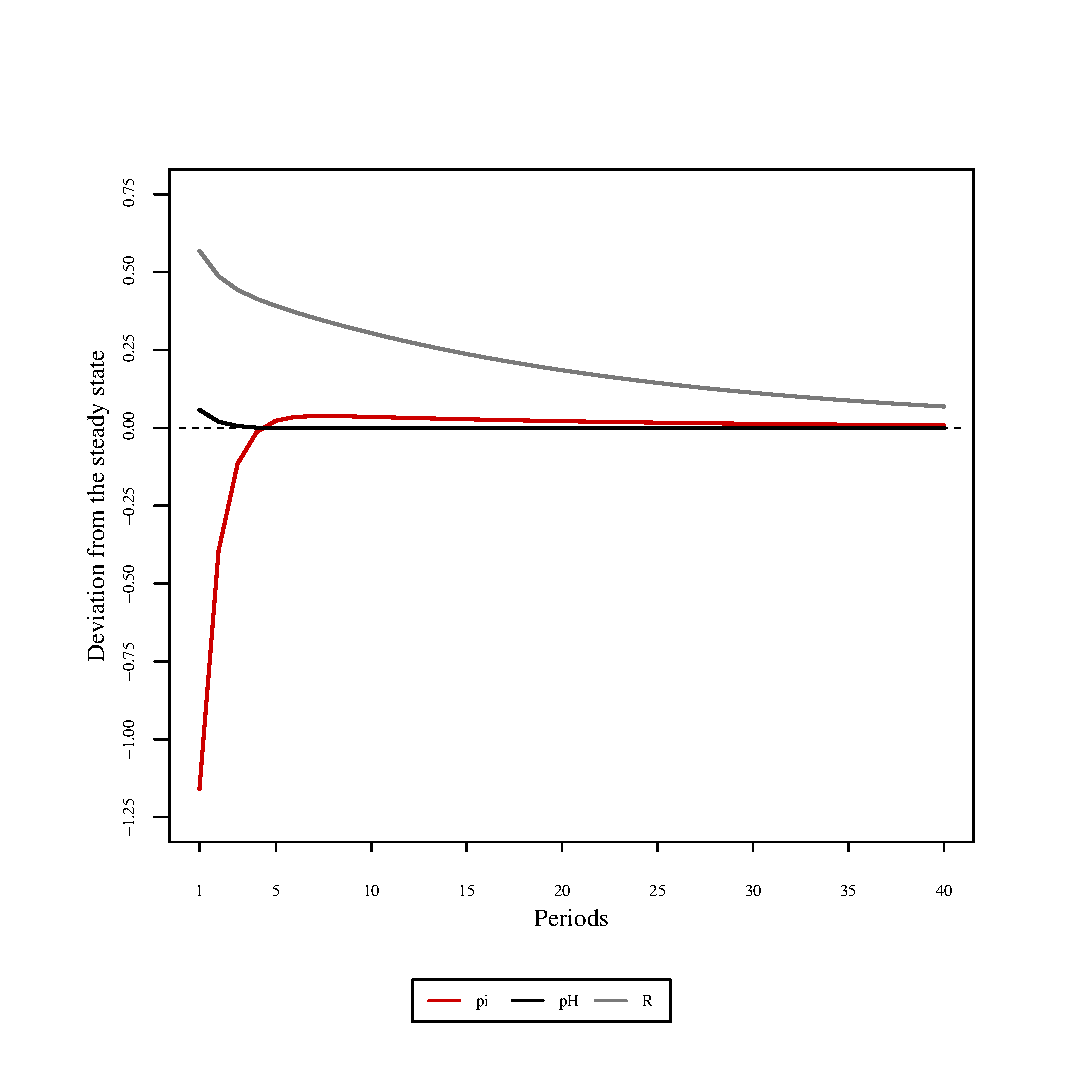
\includegraphics[width=0.99\textwidth, scale=0.55]{plots/plot_68.eps}
\caption{Impulse responses ($\pi, {p\!H}, R$) to $\eta^{\mathrm{R}}$ shock}
\end{minipage}
\begin{minipage}{0.5\textwidth}
\vspace*{-3em}
\centering
\includegraphics[width=0.99\textwidth, scale=0.55]{plots/plot_69.eps}
\caption{Impulse responses ($\pi, {p\!H}, R$) to $\eta^{\pi}$ shock}
\end{minipage}
\end{figure}

\pagebreak

\begin{figure}[h]
\centering
\begin{minipage}{0.5\textwidth}
\vspace*{-3em}
\centering
\includegraphics[width=0.99\textwidth, scale=0.55]{plots/plot_70.eps}
\caption{Impulse responses ($\pi, {p\!H}, R$) to $\eta^{\mathrm{G}}$ shock}
\end{minipage}
\end{figure}

\pagebreak

\section{Impulse response functions}

\begin{figure}[h]
\begin{minipage}{0.5\textwidth}
\vspace*{-3em}
\centering
\includegraphics[width=0.99\textwidth, scale=0.55]{plots/plot_71.eps}
\caption{Impulse responses ($\pi, {p\!H}, R, {p\!e\!r\!c\!i\!e\!v\!e\!d}^{\pi^{\mathrm{obj}}}, {i\!n\!f\!l\!a\!t\!i\!o\!n}^{\mathrm{gap}}$) to $\epsilon^{\mathrm{Z}}$ shock}
\end{minipage}
\begin{minipage}{0.5\textwidth}
\vspace*{-3em}
\centering
\includegraphics[width=0.99\textwidth, scale=0.55]{plots/plot_72.eps}
\caption{Impulse responses ($\pi, {p\!H}, R, {p\!e\!r\!c\!i\!e\!v\!e\!d}^{\pi^{\mathrm{obj}}}, {i\!n\!f\!l\!a\!t\!i\!o\!n}^{\mathrm{gap}}$) to $\eta^{\mathrm{p}}$ shock}
\end{minipage}
\end{figure}

\begin{figure}[h]
\begin{minipage}{0.5\textwidth}
\vspace*{-3em}
\centering
\includegraphics[width=0.99\textwidth, scale=0.55]{plots/plot_73.eps}
\caption{Impulse responses ($\pi, {p\!H}, R, {p\!e\!r\!c\!i\!e\!v\!e\!d}^{\pi^{\mathrm{obj}}}, {i\!n\!f\!l\!a\!t\!i\!o\!n}^{\mathrm{gap}}$) to $\eta^{\mathrm{R}}$ shock}
\end{minipage}
\begin{minipage}{0.5\textwidth}
\vspace*{-3em}
\centering
\includegraphics[width=0.99\textwidth, scale=0.55]{plots/plot_74.eps}
\caption{Impulse responses ($\pi, {p\!H}, R, {p\!e\!r\!c\!i\!e\!v\!e\!d}^{\pi^{\mathrm{obj}}}, {i\!n\!f\!l\!a\!t\!i\!o\!n}^{\mathrm{gap}}$) to $\eta^{\pi}$ shock}
\end{minipage}
\end{figure}

\pagebreak

\begin{figure}[h]
\centering
\begin{minipage}{0.5\textwidth}
\vspace*{-3em}
\centering
\includegraphics[width=0.99\textwidth, scale=0.55]{plots/plot_75.eps}
\caption{Impulse responses ($\pi, {p\!H}, R, {p\!e\!r\!c\!i\!e\!v\!e\!d}^{\pi^{\mathrm{obj}}}, {i\!n\!f\!l\!a\!t\!i\!o\!n}^{\mathrm{gap}}$) to $\eta^{\mathrm{G}}$ shock}
\end{minipage}
\end{figure}
